\newpage
\section{Accessible}
\subsection*{}
 
Los datos se consideran accesibles por el usuario cuando este no necesita realizar un esfuerzo desmesurado para
poder obtenerlos, entenderlos y usarlos, es decir, aplicarlos a su situacion particular. Para lograr estos objetivos,
es necesario que el usuario pueda acceder a ellos de una manera que le resulte familiar y en un lenguage y nomenclatura
que pueda entender.\\ 

En este apartado veremos si es posible el acceso a los datos por un usuario medio y como optimizar la accesibilidad.

\subsection{Availability}
    
As we mentioned in the introduction to this chapter, the dataSets may be available in the original source. However, this doesn't necessarily
mean that they are readily accessible.
The challenges we encounter with the raw data direct from the source of origin, are the following: \\   
 
\textbf{Location}. DataSets are usually available in open data portals that have been organized and structured in particular ways.
Despite more companies attempting to offer functional and efficient user interfaces, often a complicated search and selection process is necessary for a user to find what they need. Sometimes the data may not all be available in the one location, but may require searching through multible portals.
\textbf{Extraction}. DataSets are usually available through an API (Application Programming Interface). APIs are not easily interpretable by the average user. Normally there will be a document describing the fields and values presented, and indicating how to actually use the API. \\

\textbf{Readability}. DataSets are usually represented in a format designed to be processed by software. This is fairly unintelligible to a human user. At best,
the data will be represented in a table and even then, it will often be quite difficult to extract the required information.

Therefore, we can not say that data interfaces are commonly accessible in a useful way for the average user. \\

\subsubsection{How can we solve the problem?} 

We must provide the information required by the user in an uncomplicated manner, in a format that is easy to read and interpret, and we must describe it in a way that is easy to understand and quick to digest..

In order to collect the information which is relevant to the user, we will need to carry out processes such as extraction, transformation and
data cleaning.
 
\subsubsection{How we solve it using Aire Guru.} 

Our tool uses the air quality data provided by the city of Malaga in its open data portal.\footnote{\url{https://datosabiertos.malaga.eu/}}\\
\begin{figure}[ht]
    \centering
   \subfigure[Main page]
    {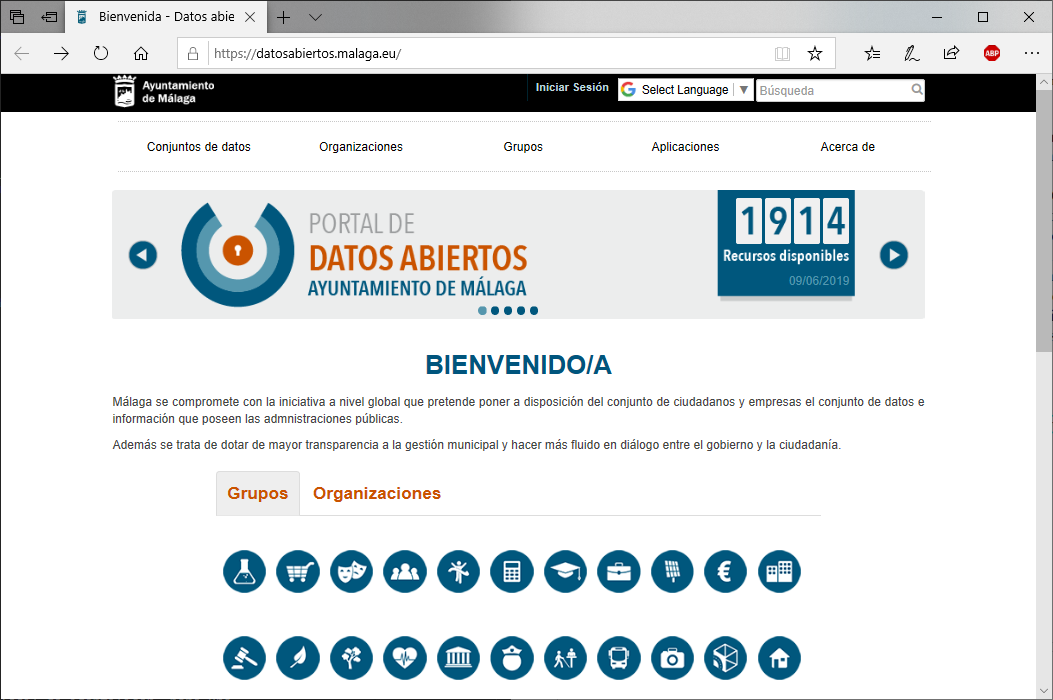
\includegraphics[width=5.5cm]{openDataPortal}}
    \hfill
    \subfigure [Category environment]
       { 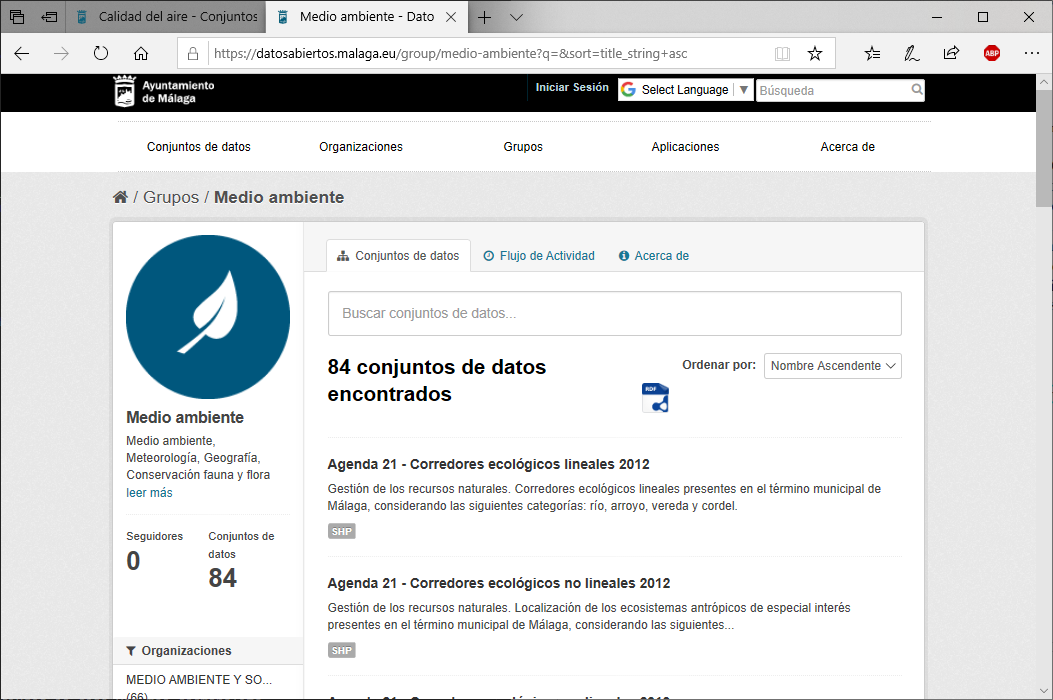
\includegraphics[width=5.5cm]{openDataPortalEnviromentCategory}}




    \vfill
     \subfigure[GeoJson Document]
     { \centering 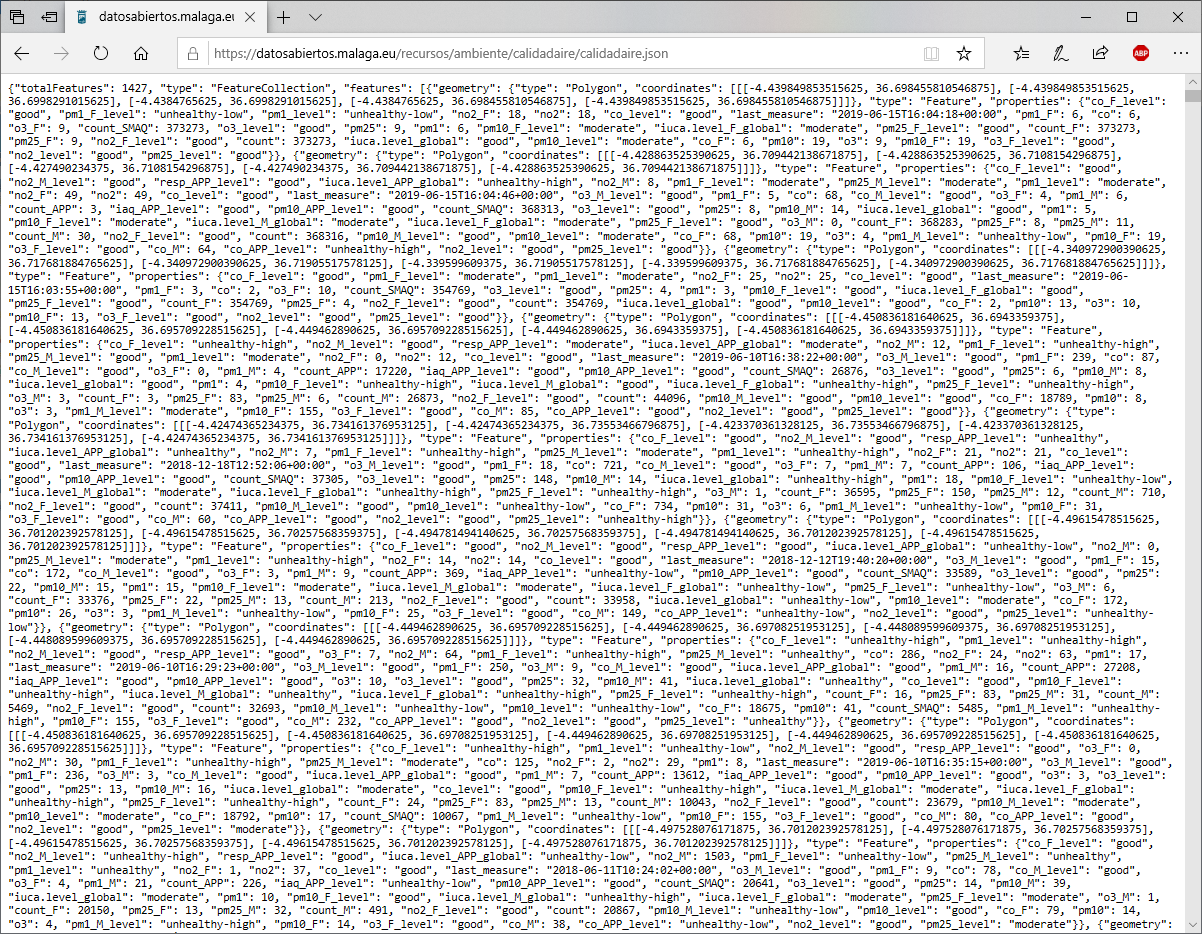
\includegraphics[width=4.75cm]{geoJsonAirQualityDataRaw}}
  
  \caption{Open Data Portal Malaga}
    \end{figure}

    This data portal offers a variety of categories (represented by different icons) indicating classifications of the dataset.
    Once a category is selected, the user is presented with a search bar that allows them to search for specific data using keywords.\\
    
    In this case, if we click on the link, data is displayed in a new tab. The use of software
    for translating the data is not strictly necessary, but we can see that the format (JSON) is not easily readable in human terms.

Aire Guru \footnote{\url{https:\\aire.guru}} offers all the necessary information on a web platform which has been designed to facilitate human understanding.

\elsparagraph{Evaluation}  

\begin{itemize}
    \done Location. Finding data is made simple, since information is displayed immediately on accessing the website. The main page
         presents the levels of pollution in all areas without the need to make any selection.
    \done Extraction. No specialist software or computer knowledge is necessary to access the information.
    \done Readability. Aire Guru includes a map which shows pollution levels, represented by different colors. These colors are defined by a legend
         below the map. It also includes a glossary explains the concepts presented on the website, the meaning of each section and includes clear instructions on how to
         use and navigate through the web page.
 

\end{itemize}
\newpage

 



\subsection{Know about}

No matter how optimized the representation of the data is and how available we make it, if users are not aware
 of the existence of the resource, they can not use it.

\subsubsection{How to solve it} 
The best way is to advertise the product in the right media with right format.
\subsubsection{How we solve it. Aire Guru} 
Our tool is implemented for the city of Malaga, so we are currently working to publicize it in this city.
It is currently available in the open data portal in the web site tab \footnote {\url {https://datosabiertos.malaga.eu/aplicaciones}} \\
Aire Guru participated in the first open data reuse contest organized by the Malaga City Council \footnote {\url {https://tinyurl.com/yx9wzutj}}
and was a finalist in the web page category.


\begin{figure}[ht]
    \centering
   \subfigure[Advertising in the open data portal of Málaga]{ \centering 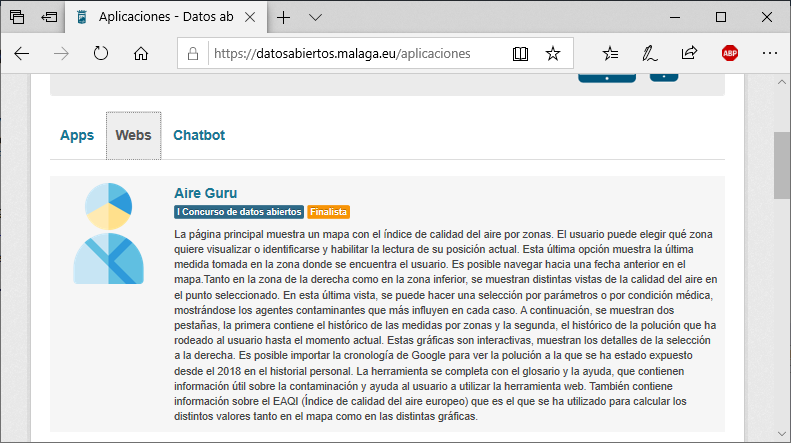
\includegraphics[width=6cm]{aireGuruFinalist}}
   \hfill
   \subfigure[Finalist]{ \centering 
\includegraphics[width=5cm]{aireGuruFinalistCertificate}}
 
    \caption{I Contest of reuse of open data. Malaga's town hall}
    \end{figure}

\elsparagraph{Evaluation}  
\begin{itemize}
    \done It is currently published in the open data portal of the City of Malaga.
\crossed More work should be done on advertising the platform and making it known.
\end{itemize}
\newpage
\subsection{Interpretabilidad}
The platforms provide a huge volume of data, since, as mentioned earlier, they collect as much data as possible.
There will be multiple samples containing the specified set of fields. These field sets may be similar to each other but don't need to be identical.
From this data, we need to select the relevant samples, and from these, the fields necessary to represent specific information.


Below we can see examples. The first one is taken from the European open data portal
\footnote{\url{https://tinyurl.com/y3d76525}} and the second from the North American open data portal
\footnote{\url{https://data.cityofnewyork.us/api/views/kku6-nxdu/rows.json?accessType=DOWNLOAD}}.

\begin{figure}[h]
    \centering
    \subfigure[EEUU Open Portal.Demographic Statistics By Zip Code]
     {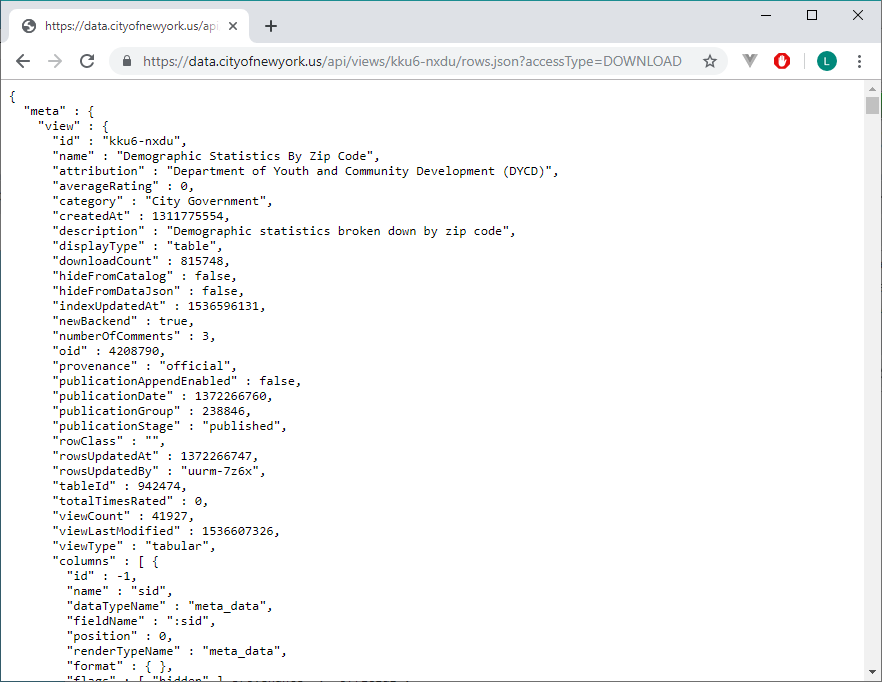
\includegraphics[width=5cm]{ExampleOpenDataEEUU}}
    \hfill
     \subfigure[European Open Data Portal. Air pollutant concentrations 2015]
    {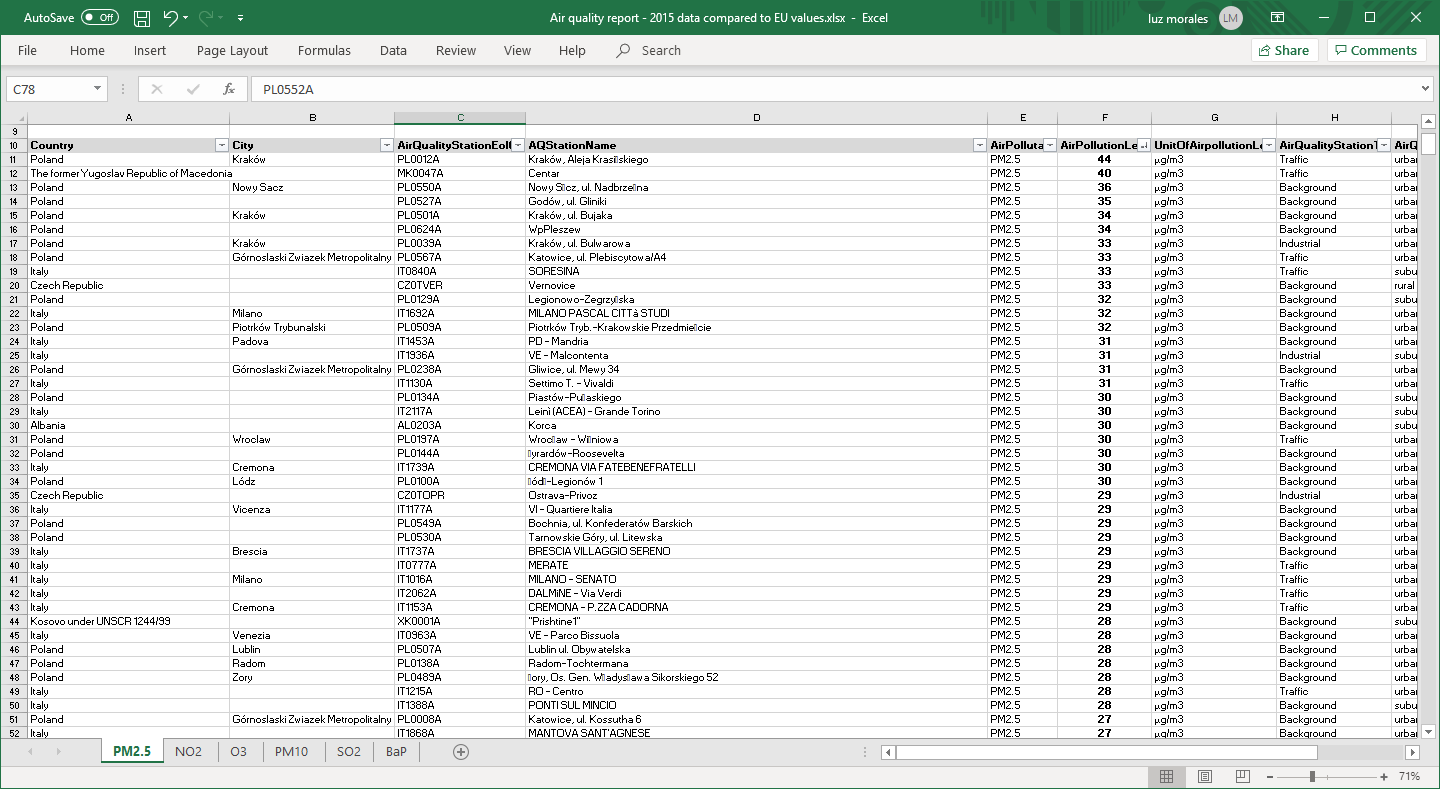
\includegraphics[width=7cm]{ExampleOpenDataEuropean}}
    \caption{Open Data Examples}
\end{figure}

    

    
\subsubsection{How to solve it} 
We obtain our required data through a series of processes such as extraction, transformation and
cleaning of the data. Without automation, theses processes are tedious and time consuming. 

\subsubsection{How we solve it. Aire Guru} 

The extracted data is in GeoJSON format, a format which provides a JSON object with nested subdocuments. Each of these
subdocuments contains a set of data in key-value form.
In the following figure we can see the beginning of the document downloaded on June 9, 2019
\footnote{\url{https://datosabiertos.malaga.eu/recursos/ambiente/calidadaire/calidadaire.json}}\\
\newpage
\begin{figure}[h]
    \centering
   \subfigure[First subdocument]{ \centering 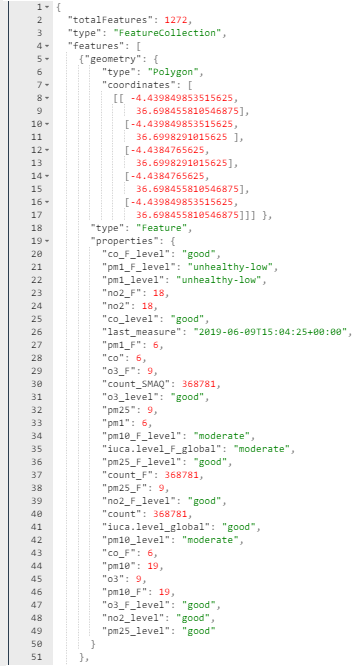
\includegraphics[width=4.75cm]{geoJsonAirQualityData1}}
   \hfill
   \subfigure[Second subdocument]{ \centering 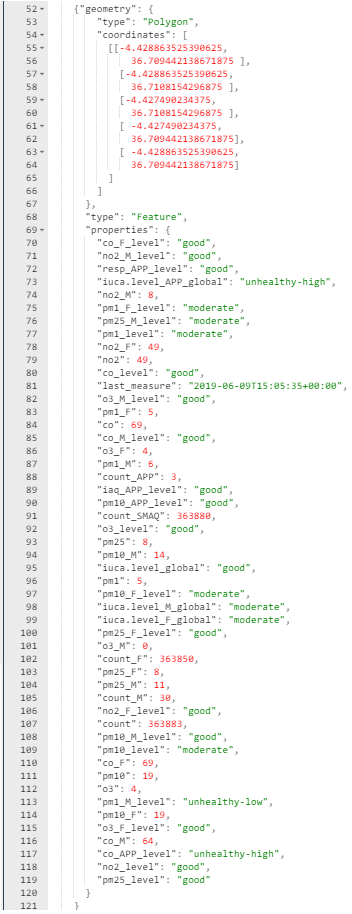
\includegraphics[width=4.75cm]{geoJsonAirQualityData2}}
 
    \caption{Air quality Document [09/06/2019].Open Data Portal Malaga}
    \end{figure}
    
    In this excerpt we can see the first two subdocuments. Each subdocument contains the coordinates of the air quality 
    measuring station, the date and time when the measurement was recorded, and the values of the measurements.
    In the following figure we can find the description provided by the open data portal.
\begin{figure}[ht]
    \centering
    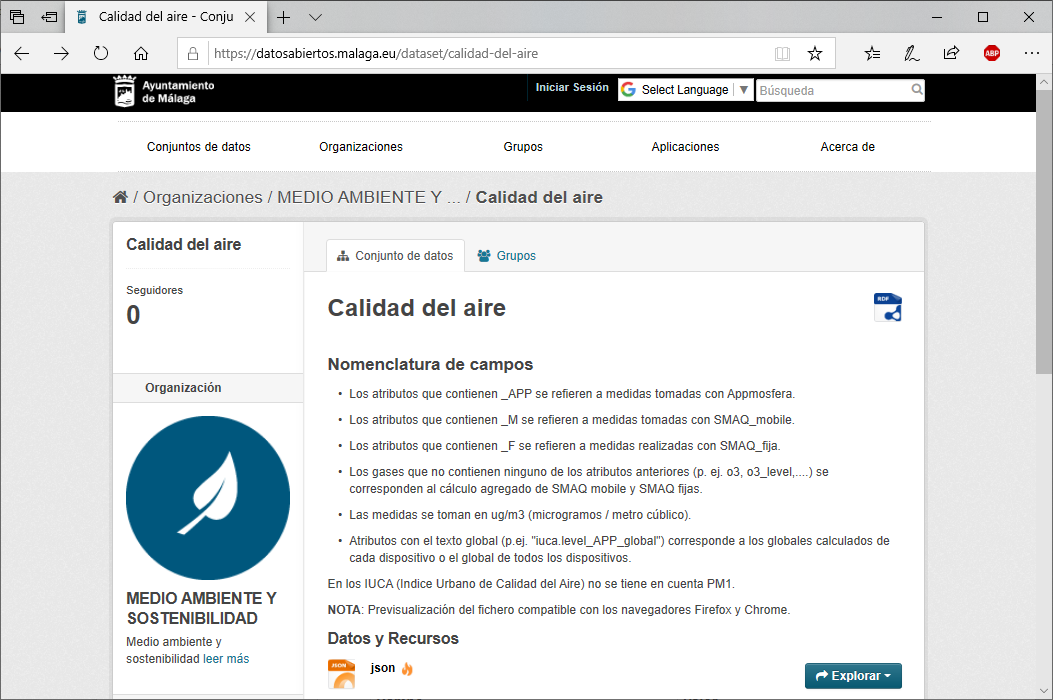
\includegraphics[width=8cm]{geoJsonAirQualityDataDescription}
    \caption{Air quality data description [09/06/2019].Open Data Portal Malaga}
\end{figure}


For a more detailed description of the measures, we have to resort to an external resource. In this case we directly contacted 
the company that installs the UrbanClouds\footnote{\url{https://urbanclouds.city/es/}} measuring stations and provides the data 
to the Malaga city council.

After selecting the necessary fields according to our design plan, we carried out different cleaning, transformation and extraction tasks. \\


\textbf{Cleaning}. We need to eliminate the repeated or non-relevant fields. For example, the identifier of the measuring station is 
unneccessary as the  already contains the coordinates of the station, and coordinate representation is more interesting for our purposes. \\

\textbf{Transformation}. We need the values to have a format appropriate to the fields that they represent. For example, the date and time 
of the measurement is stored in date format
instead of the string provided in the raw dataSet. \\

\textbf{Extraction}. We need to select the relevant fields. This dataSet offers one or more measurements for each pollutant, which can be 
represented by three different fields, a
quantitative measurement, a qualitative of the fixed station of measurement and a qualitative station of a mobile station. We will add a 
field containing the measurement which is most relevant for our purposes, and eliminate the non-relevant measurerments to minimize processing time. \\

For security, a second totally independent architecture has been implemented that collects and stores the raw data.

\paragraph{Evaluation} \mbox{} 
\begin{itemize}
    \done We can understand exactly what each one of the fields represented in the dataSet means thanks to the 
         complementary information presented in the open data portal and by the complementary information provided by the company in charge of
         collect the data.
    \done The data needed for our model has been extracted from the raw data.
    
\end{itemize}
\newpage

\subsection{Modelo}

Recall that the main objective of accessing the data is to obtain knowledge, to understand and make sense of it. Of course, 
pure data by itself has no value until we can understand it and apply it. We must contextualize, process, and analyze the 
information to gain useful knowledge. \\
    
\begin{figure}[ht]
    \centering 
    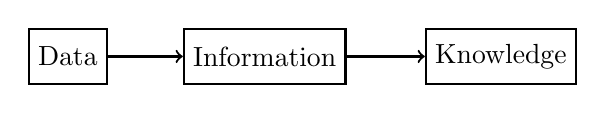
\begin{tikzpicture}[thick]
        \node[draw,rectangle,minimum size=20] (a) {Data};
         \node[draw,rectangle,minimum size=20,right of= a, node distance=2.5cm] (b) {Information};
         \node[draw,rectangle,minimum size=20,right of=b, node distance=3cm] (c) {Knowledge};
         \draw[->] (a) to (b);
        \draw[->] (b) to (c);
     
      \end{tikzpicture}
      \caption{Diagrama. De datos a conocimiento}
    \end{figure}
 
    In order to obtain this knowledge, the user must correctly interpret the data. It's not enough to know what the values and 
    units individually represent, but what they mean in the big picture. For that the user must already have expertise in the 
    area, or must engage in further research allowing them to understand the data that has been extracted.
     
    In order to build a system that makes data accessible, it is essential to design a model to specify the
    information that we want to obtain. The design of a system will allow that, based on given values, provide some results.
    For this it will be necessary to have a solid knowledge of the dataSet that is needed, the values,
    their units and how they relate to each other.


\subsubsection{How to solve it} 
Study the objective sought and resort to the help of experts if necessary to acquire the necessary knowledge
on the subject. Design a model that provides the information we are looking for.

\subsubsection{How we solve it. Aire Guru} 
Aire Guru aims to increase the awareness of the level of pollution that surrounds us. To do this, it uses a measure called
the air quality index (AQI), specifically the European air quality index (EAQI).


\newpage
\begin{figure}[ht]
    \centering
    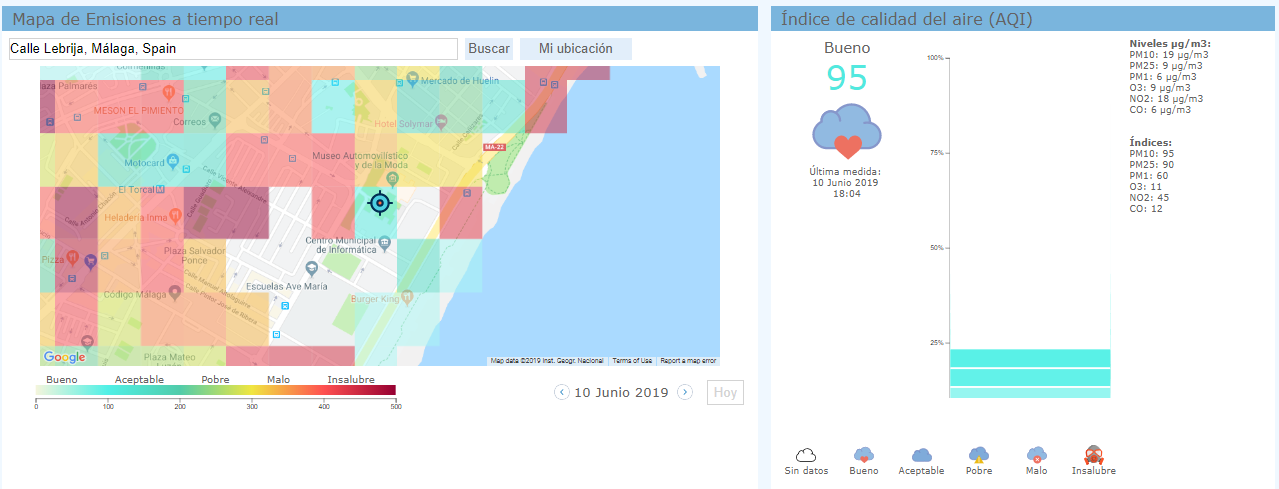
\includegraphics[width=10cm]{mapAireGuru}
    \caption{Aire Guru. Landing page. Top section}
\end{figure}

It shows the AQI in the whole city of Malaga by zones, both the general and the AQI of each of the 
pollutans in a more disaggregated form from September 2018 to the present. It also shows the evolution
of these for days, months and years.
It is capable of creating a set of the most relevant pollutans by medical condition. An innovative feature is the capacity to display levels of any particular pollutant by hour, day, month, or year. 

\elsparagraph{Evaluation}  

\begin{itemize}
\done The information is focused on an objective, informing the user of the level of pollution that surrounds them, both  in real time
and in the past.
\done The information follows a logical thread; it tells a story.
\done The web offers understandabl, useable information, not just raw data.
\end{itemize}

\newpage
\subsection{Formato}
El punto clave para que el usuario entienda lo que queremos transmitirle es crear una comunicacion fluida entre la representacion
de los datos el usuario. Para ello  deberemos asegurarnos que hablamos el mismo idioma, con un vocabulario facil de entender y
con proximidad, es decir,dejar la terminologia a un lado y comunicar el objetivo de la manera mas simple posible.
Por ello la representacion de la informacion jugaran un papel fundamental para que la 
informacion sea absorbida por el usuario de una manera natural.


\subsubsection{How to solve it} 
Este modelo debera proporcionar la informacion al usario en un lenguaje o formato compresible. Si no es posible proporcionaremos las 
herramientas necesarias para que este pueda comprender el contexto de la informacion.
Deberemos estudiar que tipo de representacion es mas adecuada, no siempre una grafica es la representacion mas adecuada, deberemos hacer un 
estudio de tanto al publico al que va dirigido como como podemos acentuar la informacion que sea mas relevante en la manera 
correcta.
Si nos declinamos por realizar una representacion con graficas, deberemos estudiar los datos para saber que tipo de grafica. Por ejemplo, 
si hablamos de muestras y queremos saber la densidad, nos inclinaremos por un grafico de densidad y si por ejemplo buscamos la diferencia 
entre sexos, utilizaremos un grafico de tartas.

\subsubsection{How we solve it. Aire Guru} 
La herramienta Aire guru presenta la informacion en el idioma nativo de la ciudad y se utiliza un lenguaje sencillo y directo.
See utiliza el mismo estilo, colores e iconografia en todo el diseno para que el usuario se familierize rapidamente y pueda
prestar atencion al significado de los datos en vez de perderse en el diseno e intentar encontrar su significado.//

Unos de los objetivos es representa la contaminacion por zonas de la ciudad, por lo que se ha utilizado un mapa sobre el que se representa
 el AQI general calculado. Este es un formato mas legible para los usuarios ya que no tiene que trabajar para realizar una imagen visual
 de los distintos lugares de la ciudad. Este indice mustra un indicador con cinco niveles representados por una escala de colores desde el 
 turquesa hasta el rojo ("Bueno" "Aceptable""Pobre" "Malo" e "Insalubre"). La razon de esta eleccion es porqu eson los colores oficiales y 
 asi se evita crear confusion al usuario.
 \newpage
 \begin{figure}[ht]
    \centering
    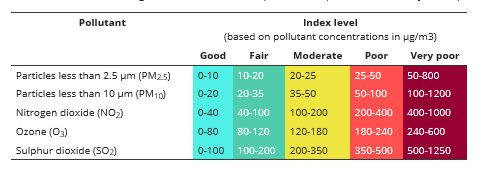
\includegraphics[width=12cm]{EAQI}
    \caption{EAQI Levels}
\end{figure}

Nuestra plataforma introduce ademas una iconografica para ayudar al usuario a tener una idea directa de la situacion, ya que son mas 
explicativos que los colores. En caso de peligro, queda bien representado con el color rojo, pero en el caso del azul o verde, en nuestra cultura, no
tenemos definido un estado para estos colores.\\
\begin{figure}[ht]
    \centering
    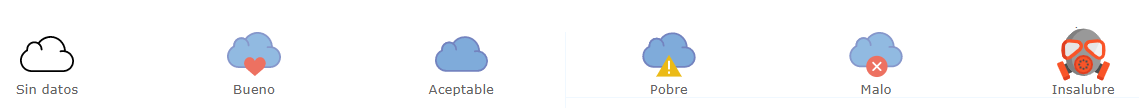
\includegraphics[width=10cm]{EAQI_Icons}
    \caption{Iconografica Aire Guru}
\end{figure}

Para las graficas que muestran variaciones en el tiempo, se han utilizado graficos de lineas, que son las mas apropiadas para este tipo de datos,
ya que muestran la continua evolucion durante un periodo de tiempo. Para representar los distintos componentes del AQI se ha utilizado un
grafico de barras apiladas, ya que se ve que proporcion del AQI total esta formada por que contaminante.\\
\begin{figure}[ht]
    \centering
    \subfigure[AQI Evolution]
     {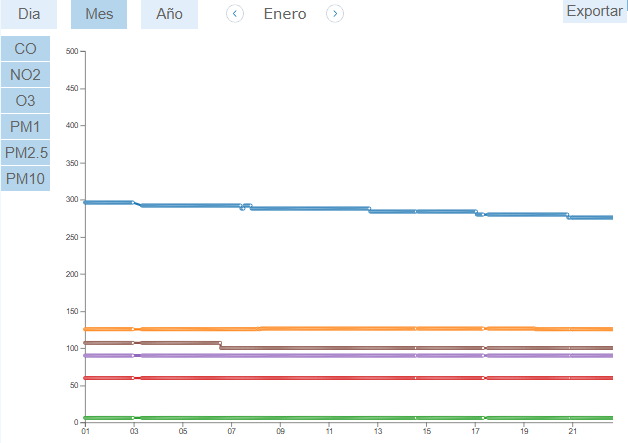
\includegraphics[width=5.75cm]{lineChart}}
     \hfill
     \subfigure [AQI components]
    { 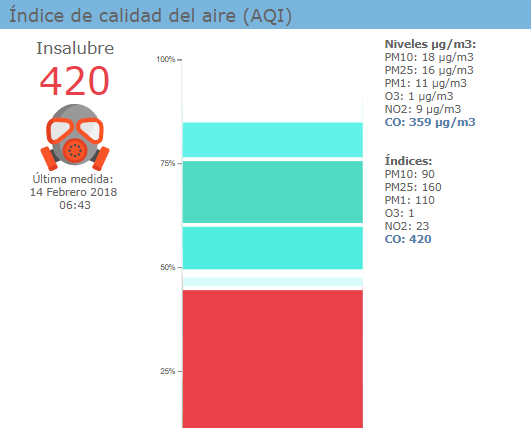
\includegraphics[width=5.25cm]{stakedBarChart}}
 
    \caption{Charts}
\end{figure}

Ademas, para explicar el concepto de AQI y crear un awarnes sobre la influencia que tiene en nosotros la polucion del aire, Aire Guru proporciona un 
glosario y una ayuda con las descripciones de los agentes contaminantes, complicaciones medicas, fuentes de contaminacion, la iconografia utilizada y
una explicacion sobre que es y como se calcula el AQI.\\

 
\elsparagraph{Evaluation}  
\begin{itemize}
    \done El lenguaje utilizado en toda la herramienta es un lenguaje comun, huye de la terminologia cientifica pero proporciona la informacion
    suficiente para enteder la situacion.
    \done Se han estudiado y utilizado las graficas mas apropiadas para cada tipo de datos.
    \crossed Algunos terminos especificos no se han podido sustituir como "Indice de calidad del Aire".
    \done Se han proporcionado la herramientas necesarias para entender el concepto. Se ha utilizado la norma europea de calidad del aire para 
    representar los valores y se ofrece al usuario recursos en la pagina para su comprension ademas de recursos extenos.
    
\end{itemize}
 

\newpage
\subsection{Convenience}
As we mentioned earlier, our goal is for the user to have direct access to the data without having to deal with any
of the technical processes involved in implementing a collection system. The points we must cover to achieve this goal are: \\

\textbf{Infrastructure}. Data collection, processing, storage and visualization. For example, in most cases, the data is
published periodically, but the set of published data only contains the most recent samples. There is no way to obtain
a history of the data if it is not collected, processed and stored periodically. \\

\textbf{Automation}. As we commented in the previous point, these tasks are repetitive and arduous processes, so it will be
necessary to automate, otherwise the effort required by the user to extract the information is not worthwhile. \\

\textbf{Availability} To offer the information to users in a direct way, we should use a platform with which the user is already 
familiar. For example, it is more likely that the user will want to access the data if there are no extra obstacles such as needing 
to install new software on their devices. \\

\subsubsection{How to solve it} 
We will have to provide all the afore-mentioned infrastructure which can collect the data and offer it to the user in an accessible, relevant and compelling way.
We will try to free the user from repetitive actions, we will automate all possible processes, to make the information available immediately.
We must offer the information through a platform with which the user is familiar, nowadays the use of websites or mobile applications is very common.
We must not make the user perform complicated steps, or require them to add extra software or hardware.

\subsubsection{How we solve it. Aire Guru} 
Malaga's air quality dataset is updated every hour, Aire Guru automates the process of collecting the
data through a CRON job that executes a script implemented in JavaScript periodically. This reads the data from the url, processes it,
cleans and stores it in a MongoDB database. That is to say, Aire Guru implements all the necessary collection processes.

Thanks to this infrastructure, the user is able to visualize the evolution of pollutants since 2018. The user can also track their personal exposure
 to these pollutants over the same period of time.

In addition, this automation allows the user to visualize the pollution in the city of Malaga in real time, and see specifically the location where he is 
occurring. \\
\newpage

\begin{figure}[ht]
    \centering
    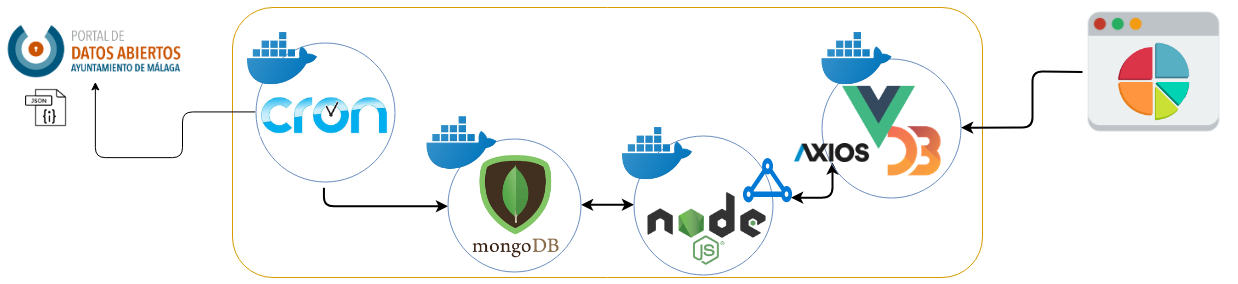
\includegraphics[width=12cm]{aireGuruArquitecture}
    \caption{Arquitecture Aire Guru}
\end{figure}

The data to the users through a web interface. \\

\begin{figure}[ht]
    \centering
    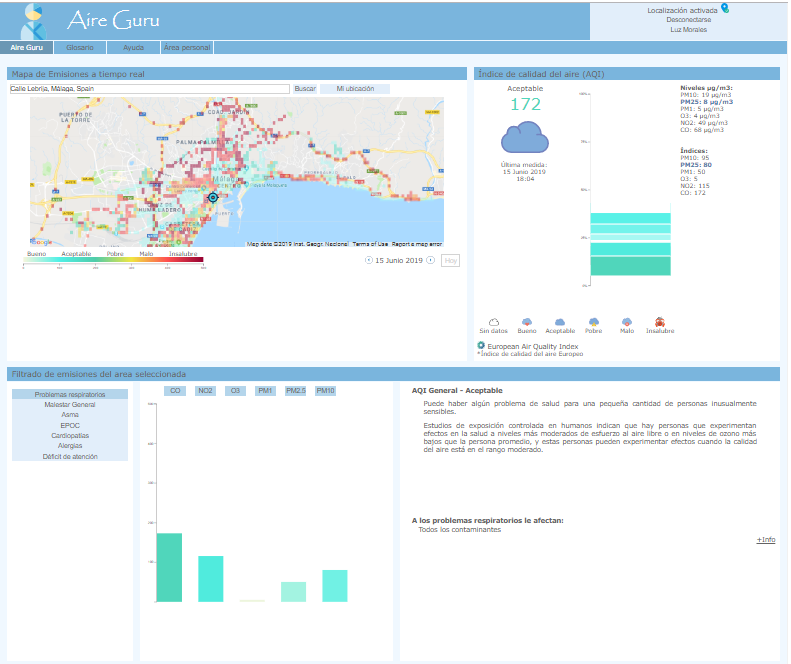
\includegraphics[width=9cm]{aireGuru}
    \caption{Aire Guru. Web Interface}
\end{figure}

To enable access by the majority of the population, Aire Guru is available at the web addresses https://www.aire.guru and https://www.airquality.guru.
We use SSL that guarantees the encryption of data through the network and ensure the user has access to it since, as more and more browsers try to protect 
users by only showing pages that use a secure method.

As we commented previously, all users can see the basic information without having to provide any data or identify themselves, without the need to
perform downloads or installations. Today, almost everyone is familiar with web browsing and if we do not force the user to realize extra taks, as 
requiring them to sign in or install extra software, the probability the user uses our platform will be higher. 

\newpage
\elsparagraph{Evaluation}  
\begin{itemize}
\done The data necessary for our model has been extracted from the raw data.
\done Infrastructure. Aire Guru implements all the necessary architecture of storage, processing and visualization so that the user only has to consult
the data.
\done It automates the processes of data collection and the necessary calculations to show the information to the user.
\done It offers users a free web page, and facilitates the users direct access to information.
\end{itemize}


\subsection{Optimizacion de la accesibilidad}

Para ofrecer los datos a los usuarios de una manera directa, es recomendable utilizr una plataforma a la que el usuario
este familiarizado. Por ejemplo, es mas factible que el usuario se sienta mas atraido a acceder a los datos si no requiere
ninguna instalacion en sus dispositivos.\\

-- Instalacion de dispositivos para extraer la informacion ellos mismos


\subsubsection{How to solve it} 
Ofrecer la informacion mediante una pagina web o una aplicacion movil. Ofrecer toda la informacion posible sin necesidad de
hacer que el usuario realize acciones complicadas, como la identificacion.
Ofrecer una plataforma segura.

\subsubsection{How we solve it. Aire Guru} 

Para garantizar el alcance a la mayoria de la poblacion, Aire Guru esta disponible en las direcciones webs https://www.aire.guru y https://www.airquality.guru.
Usa SSL que garantiza la encriptacion de los datos atraves de la red, ademas, cada vez mas navegadores intentan proteger a los usuarios y
solo muestran paginas que utilizar un metodo seguro. 

Como comentabamos anteriormente, todos los usuarios pueden ver la informacion basica sin necesidad de aportar ningun dato o identificarse, sin la necesidad de 
realizar ninguna descarga o instalacion y hoy en dia, casi todo el mundo esta familiarizado con la navegacion web.

\elsparagraph{Evaluation}  

Ofrecerles a los usuarios una pagina web libre de cargos, facilita que el usuario acceda directamente a la informacion
sin tener que realizar ninguna descarga. Al eliminar esta barrera, el usuario nos da un punto de confianza.
--reacio a identificarse
--y actualmente se esta trabajando en su traduccion al ingles, para cubrir un rango mas amplio de su poblacion, ya que esta ciudad es cada vez mas cosmopolita.
\\newpage

\begin{figure}[ht]
  \centering
  \framebox{
  \vbox{\begin{tabbing} 
  Check List \\
  \hspace*{10mm} \ding{47} Point 1 \hspace*{25mm} \= \ding{47} Point B \\
   
  \end{tabbing}}%
  
  }
  \end{figure}

    
